\chapter{Deep Networks for CFO}

\section{Recurrent Neural Network Follows a Circle}

\setlength{\tabcolsep}{0pt}
\begin{figure}
  \centering
  \caption{Linear neural network: follow a circle for a constant CFO rate.}
  \begin{tabular}{ccc}
    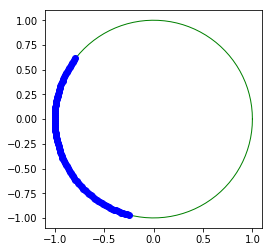
\includegraphics[width=50mm]{figures/follow_circle_linear_before.png}&
    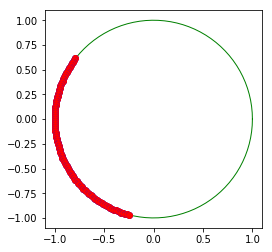
\includegraphics[width=50mm]{figures/follow_circle_linear_after.png}&
    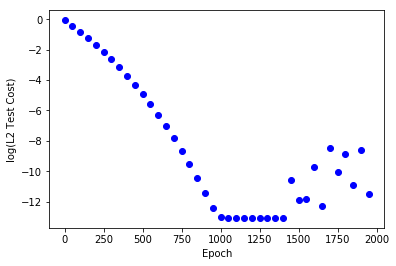
\includegraphics[width=70mm]{figures/follow_circle_linear_loss.png}\\
  \end{tabular}
  \label{fig:circle_constant_rate}
\end{figure}

Figure~\ref{fig:circle_constant_rate} shows a recurrent neural network (RNN) that follows a circle for a constant rate of rotation.  The network has input of the starting points, $x[0]$, and must predict the next $100$ points, $x[1] \ldots x[99]$.  Point $x[i]$ is rotated by $e^{ij\omega}$ where $\omega$ is the rate of rotation.  The RNN architecture is one linear layer that takes the current point as input, $x[i]$, and outputs the next point, $x[i+1]$.  We use a linear layer here because the network essentially has to learn how to become the rotation matrix.

\begin{align}
R = \begin{bmatrix}
cos(\omega) & - sin(\omega) \\
sin(\omega) & cos(\omega)
\end{bmatrix}
\end{align} 



\setlength{\tabcolsep}{0pt}
\begin{figure}
  \centering
  \caption{Nonlinear neural network: follow a circle for a different CFO rates.}
  \begin{tabular}{ccc}
    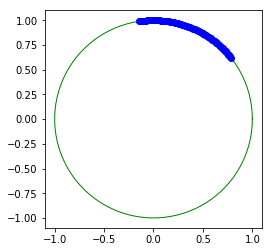
\includegraphics[width=50mm]{figures/follow_circle_nonlinear_before.png}&
    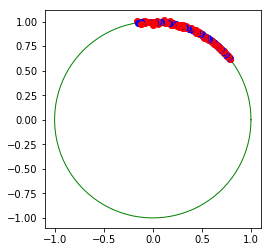
\includegraphics[width=50mm]{figures/follow_circle_nonlinear_after.png}&
    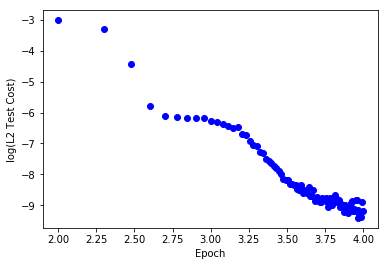
\includegraphics[width=70mm]{figures/follow_circle_nonlinear_loss.png}\\
  \end{tabular}
  \label{fig:circle_diff_rate}
\end{figure}

for a constant rate
for a given rate


\section{Deep Network Carrier Frequency Offset Estimation}
\begin{itemize}
\item complex gradients problems
\item act like the real and imaginary parts are separate
\item plots: one tap channel plots, without equalization problems
\item plots: two tap channel plots, with equalization problems
\end{itemize}


\begin{figure}
\begin{center}
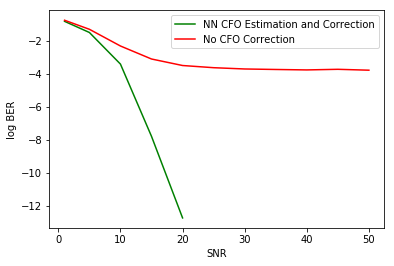
\includegraphics[width=14cm]{figures/cfo_estimation.png}
\caption{The log BER of received signals passed through a neural network CFO estimator with a rotation matrix CFO correction and classic demodulator. The log BER of the same signals passed through just the classic demodulator.}
\label{fig:cfo_est}
\end{center}
\end{figure}

Figure~\ref{fig:cfo_est} shows how...

\section{Deep Network Carrier Frequency Offset Correction}
Program a Costas loop for comparison 